\section{縫い目形状のモデリングと移動境界条件}
\label{sec:geometry-boundary}

\subsection{縫い目形状のパラメトリックモデリング}
\label{sec:seam-geometry}

野球公式球そのものの実測STL/CADデータで自由に利用できるものは見つからなかった（メーカーの内製図面が非公開のため）。一方，CFD文献では公式球の実測諸元（円周・縫い目高さ等）に基づき，縫い目を「球面上を二重らせん状に周回する1本の曲線＋隆起した断面形状（バンプ断面）」として簡略化してモデル化する手法が広く使われている\cite{iop_seam_cfd}。本プロジェクトでも同様の方針を採用する。

\paragraph{縫い目中心線}
球面上を，方位角1周あたり緯度が2回振動する閉曲線として生成する（\texttt{src/geometry/seam.jl}）：
\begin{align}
	\frac{z}{R} = A\sin(2u), \qquad \phi = u, \qquad u\in[0,2\pi).
	\label{eq:seam-curve}
\end{align}
振幅 \(A\)（縫い目が到達する最大の \(|z|/R\)）が唯一の形状調整パラメータであり，暫定値は\(0.7\)。単純な式だが，実球の縫い目が持つ次の性質を満たすことを確認済みである：自己交差のない単一閉曲線であること，球面を合同な2枚の二葉（ピーナッツ形）に分割すること（\(x\)軸まわり\(180^\circ\)回転が2枚を入れ替える——実際の2枚革と同じ），そして\(z\)軸回転では1回転あたり4本，\(x\)/\(y\)軸回転では2本の縫い目が気流を横切ること——これが4シームと2シームの幾何学的な違いそのものである。

\begin{figure}[H]
	\centering
	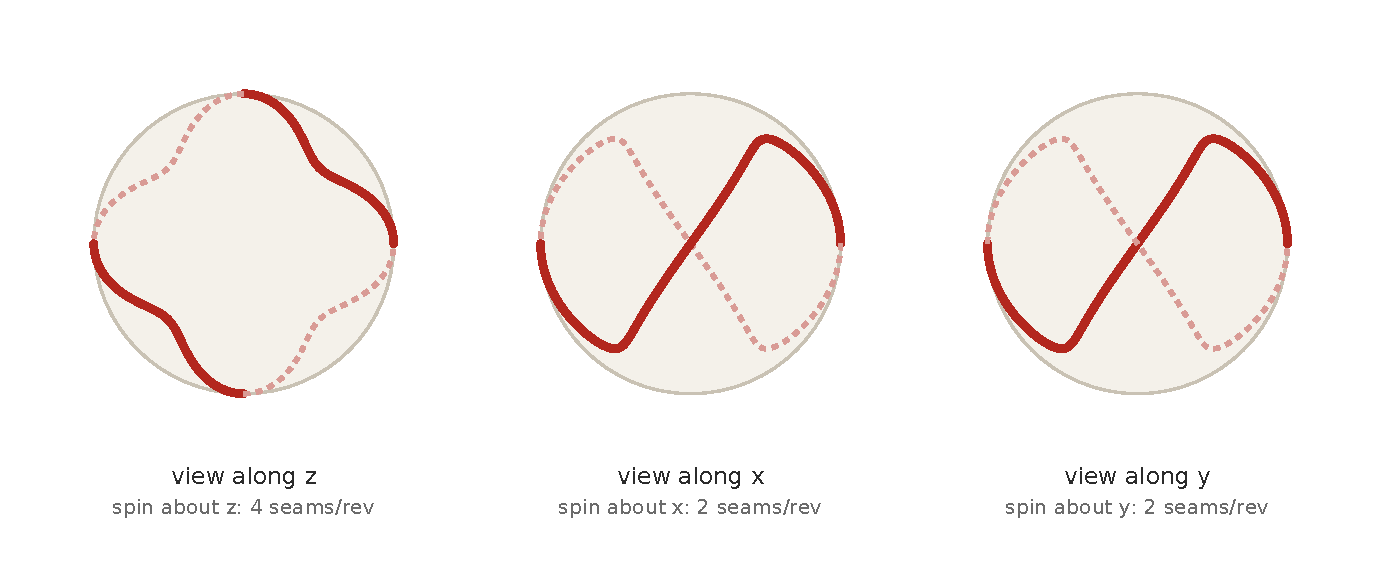
\includegraphics[width=0.95\textwidth]{figure/seam.pdf}
	\caption{パラメトリック縫い目モデル（\(A=0.7\)）の3方向からの投影。実線が手前，破線が奥。\texttt{scripts/plot\_seam.jl}で再生成できる。}
	\label{fig:seam}
\end{figure}

\paragraph{断面形状}
縫い目曲線を中心線とする半径 \(h\) の円管とする。中心線が球面上にあるため，管は球面から外側へちょうど \(h\) だけ隆起する。高さは実測値に基づき既定0.79\,mmとする。

\paragraph{符号付き距離関数（SDF）化}
球と縫い目チューブの和集合の符号付き距離関数として実装する（\texttt{src/geometry/sdf.jl}）：\(\min(\text{球のSDF}, \text{チューブのSDF})\) で評価する。これは固体外部では厳密な距離，内部では保守的な下界となるが，境界処理が必要とするのは外部側の距離のみであるため問題にならない。格子上への事前計算では，縫い目の寄与が効く表面近傍のみ（既定で表面から \(h+3\Delta x\) 以内）で縫い目距離を評価し，遠方は球のSDFで済ませる。

\subsection{移動境界の境界条件}

球は角速度 \(\vec\omega\) で自転する。密結合方式（\secref{coupling}）では計算領域はボールに追従する並進座標系に固定されるため，境界条件としては「その場での自転」のみを扱えばよく，並進運動はフレーム側で吸収される。

\begin{itemize}
	\item \textbf{基本手法}：補間バウンスバック法（Bouzidi/Yu型 interpolated bounce-back）を用い，格子点と実際の球面（縫い目を含む）との交点位置に応じてサブグリッド精度で反射則を補間する。
	\item \textbf{表面速度条件}：境界上の各点で \(\vec u_{wall}=\vec\omega\times\vec r\) を課し，回転による運動量を流体側へ正しく伝達する。
\end{itemize}

\subsection{力・トルクの評価}

球表面上の運動量交換則（Momentum Exchange Method, MEM）により，格子ボルツマンの粒子分布から直接，球に働く圧力抵抗・摩擦抵抗・揚力・トルクを運動量収支として算出する。これにより解析式に頼らず，流体場から一貫して瞬時の \(\vec F_{aero}\)，\(\vec T_{aero}\) を得る。

\subsection{回転する縫い目球と局所再カット}
\label{sec:recut}

回転境界条件は \(\vec u_{wall}=\vec\omega\times\vec r\) を課すが，これは滑面球には十分でも縫い目球には足りない——球は回しても同じ形だが，縫い目球は向きによって形が変わる。しかも縫い目は到達可能などの解像度でもサブセル（1格子間隔未満）の特徴であるため（\secref{resolution-budget}），ソルバから見た「縫い目」の実体は補間バウンスバックの距離パラメータ \(\delta\) そのものである。\(\delta\) を固定したままでは，静止した模様を着た滑面球を解いていることになる。

ボール追従座標系ではボールは並進せず，かつ球は回転対称であるため，分類が変わりうる節点の集合は向きによらない薄いシェルに固定される：球の内部（\(\varphi_{sphere}<0\)）は縫い目チューブが和集合として加わるだけなので常に固体，球面から十分離れた外側（\(\varphi_{sphere}>h+\sqrt3\)）はチューブの隆起もバウンスバックのリンクも届かないため常に流体である。その間だけがシェルであり，再カット（自転に伴う固体・流体分類の更新）の対象となる。境界節点の列番号は初期化時に一度だけ割り当てられ，再カットは値の上書きのみで完結する。

縫い目の対称性（\(u\to u+\pi\)すなわち\(z\)軸まわり\(180^\circ\)回転で自己一致）を用いた検証では，その向きでの再カット結果が元のカットとビット単位で一致することを確認しており，探索・シェル番号付け・二分法のいずれもこの対称性を壊していないことの強い証拠となっている。

再カットが必要な頻度は，1ステップあたりの赤道での表面移動量（格子間隔単位）
\begin{align}
	\omega\,\Delta t\,\frac{R}{\Delta x} = \frac{\omega R}{U}\,u_{lattice} = S\,u_{lattice}
	\label{eq:recut-rate}
\end{align}
から決まり，\(\Delta x\)に依存しない——\textbf{スピンパラメータと格子マッハ数だけで決まる}。本プロジェクトの検証ケース（\(S=0.272\)，\(u_{lattice}=0.05\)）では0.0136格子/ステップであり，1/4格子ごとに再カットするなら18ステップおきでよい。これが密結合ループ（\secref{coupling-loop}）のサブサイクル長の上限を決める。
